\chapter{Introduction}
Maintenance scheduling is in its nature a multi actor process. Many stakeholders have to coordinate in both time and space to allow for an
efficient and effective execution. This thesis will propose a generalized multi-agent scheduling system and it will argue that for the field of
maintenance scheduling to more forward similar approaches will have to be adopted. Other approaches may be very different but they will share many 
of the aspects. 

This Ph.D. will present a generalized dynamic multi-model approach to maintenance scheduling which will be model after a practical maintenace handbook \cite{palmer_maintenance_2019}.
This book written by the experienced practitioner Richard D. Palmer will be a guiding light throughout the thesis, so it serves as the main source and validation, 
or maybe invalidation is a better word, as we explore the academic maintenance scheduling literture and also, and more importantly, it will also be the source 
which above all else will us us through the perilous process of create a generalize model setup for maintenance scheduling.



\section{The General Maintenance Scheduling Process}
This section will provide an overview of the maintenance scheduling process in the most abstracted way possible. It will be important to understand this setup
throughly as most industries that perform maintanance of a considerable scale follow this process. Many industries are of course unique and deviate
from general framework in specific work but the fundamentals are usually quite similar. 

\begin{figure}[H]
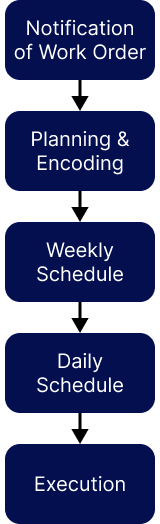
\includegraphics[width=1.0\textwidth]{figures/top-level-schedule-overview.png}
\label{top-level-schedule-overview.png}
\end{figure}





\chapter{Modelling the Generalized Setup}
To model the maintenace process in its entirety we will need tool that are powerful enough to describe the system. The system will be described in accordance 
with the \ref{top-level-schedule-overview.png} \cite{palmer_maintenance_2019}.

The maintenance scheduling problem is NP-hard and real-time optimal solutions will never be a feasible approach unless we use a multi-model setup where each model enriches the 
overall solution in the way that it is most capable of. 
